\documentclass[11pt]{article}
\usepackage{url}
\usepackage{cite}
\usepackage{amsmath}
\usepackage{graphicx}
\graphicspath{{../umlet/}}

\begin{document}

\title{Notes}
\author{Ernest Kirstein}
\maketitle

\section{Recursive Descent Parsing}
\label{rdp}
Historically, recursive descent parsers have been coded manually or else compiled from 
a context free grammar specification. \cite{compiler} 
Coding a RDP manually is tedious and error prone.
Compiling a context free grammar into a recursive descent parser
may not preserve the {\em strong equivalence} of the grammar
since some grammars need to be manipulated before
they can be parsed by a RDP. This makes any manipulation of the
resulting parse trees much more difficult. 

In this paper, I will describe a novel approach to recursive descent parseing
which solves both problems by first compiling a grammar into a recursive descent
parseable grammar, then decompiling the parse trees generated from the RDP back into
the initial grammar.


\subsection{What does a Recursive Descent Parser Do?}
The introductory material by Dr. Lewis \cite{lewis} describes a RDP as a piece of software which takes 
a sentence and puts it into a parse tree by performing a 'depth-first' search. 
But a search of what? One might try to call it a search of the derivation (parse) tree, but that's not exactly right.
The 'recursive descent' name comes from the nature by which an RDP traverses through a
syntax diagram of a context free grammar \cite{compiler}. 
But looking at only the syntax diagram, rather than the
grammar directly, one might the relationship between the
RDP search and the grammar rules.
This section will describe a different way of visualising a recursive descent parser's path,
which I have not found in the literature.

Consider a context-free grammar with the following production rules:
\setcounter{equation}{0}
\begin{align}
S &\rightarrow a S\\
S &\rightarrow b S\\
S &\rightarrow \epsilon
\end{align}
And the following string which we will attempt to parse: "ab"

We know, right off the bat, that the start symbol $S$ will be the root of any parse tree created under this
grammar, by virtue of it being the start symbol. (Figure \ref{fig:rdp_0})

\begin{figure}[h!]
    \centering
    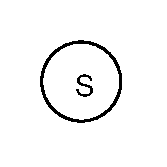
\includegraphics[natwidth=15,natheight=15]{rdp_0.pdf}
    \caption{Parse Tree 0}
    \label{fig:rdp_0}
\end{figure}

The next parse tree we should consider is the parse tree that is generated when we follow the first 
production rule. (Figure \ref{fig:rdp_1}) Notice that, in this instance, the parse tree does not conflict with
the string we are trying to parse - i.e. regardless of the production rules we follow the string that is
produced from any further production rules we follow will start with "a".

\begin{figure}[h!]
    \centering
    \includegraphics[width=0.4\textwidth,natwidth=30,natheight=30]{rdp_1.pdf}
    \caption{Parse Tree 1 - Valid}
    \label{fig:rdp_1}
\end{figure}

For the next parse tree, we will try to repeat are last action (following the first possible production rule).
(Figure \ref{fig:rdp_2}) This parse tree conflicts with the string we are trying to produce since any
string produced by further production rule applications will produce a string starting with "aa".
In this case, we go back to the previous parse tree and try a different production rule.

\begin{figure}[h!]
    \centering
    \includegraphics[width=0.4\textwidth,natwidth=30,natheight=30]{rdp_2.pdf}
    \caption{Parse Tree 2 - Invalid}
    \label{fig:rdp_2}
\end{figure}

In figure \ref{fig:rdp_3}, we've followed the second production rule
and our new parse tree fits with the input string, so we can continue our descent.

\begin{figure}[h!]
    \centering
    \includegraphics[width=0.4\textwidth,natwidth=30,natheight=30]{rdp_3.pdf}
    \caption{Parse Tree 3 - Valid}
    \label{fig:rdp_3}
\end{figure}

The next two parse trees (Figure \ref{fig:rdp_4_5}), created by applying the first and second production rules to
Parse Tree 3, are both invalid because they extend past the length of our input string.

\begin{figure}[h!]
    \centering
    \includegraphics[width=0.4\textwidth,natwidth=30,natheight=30]{rdp_4.pdf}
    \includegraphics[width=0.4\textwidth,natwidth=30,natheight=30]{rdp_5.pdf}
    \caption{Parse Trees 4 and 5 - Both Invalid}
    \label{fig:rdp_4_5}
\end{figure}

At the last step, by applying the third production rule to Parse Tree 3, we have a parse tree which terminates and produces the
desired input string, "ab". (Figure \ref{fig:rdp_6})

\begin{figure}[h!]
    \centering
    \includegraphics[width=0.4\textwidth,natwidth=30,natheight=30]{rdp_6.pdf}
    \caption{Parse Tree 6 - Complete}
    \label{fig:rdp_6}
\end{figure}

Finally, let's diagram our traversal through the possible parse trees (Figure \ref{fig:rdp_7}). Shown this way, it becomes quite
clear that what a recursive descent parser does - it performs a depth first search of the graph of possible parse trees, looking
for a parse tree which fits the input string, where the child nodes from each PT node in the graph are PT nodes generated by
applying each of the production rules to the first nonterminal symbol in that PT node. The depth of each node in the PT graph
corresponds with the number of terminal symbols (including the empty string) that have been parsed.

\begin{figure}[h!]
    \centering
    \includegraphics[width=0.4\textwidth,natwidth=30,natheight=30]{rdp_7.pdf}
    \caption{Parse Tree Search Progression}
    \label{fig:rdp_7}
\end{figure}

\clearpage

\subsection{Compiling and Decompiling a Context Free Grammar for RDP}
The core rules for my parser are built off of Dr. Lewis's notes \cite{lewis}.
A grammar is define as an ordered collection of production rules.
My parser uses context-free grammar rules, which are comprised of a
'head' (the single-symbol left hand side of the production rule), and a 'tail'
(one or more symbols comprising the right hand side of the production rule).

These grammars may be 'compiled' using the four procedures:
factoring, substitution, removing left recursion, and removing useless
rules. Let 'decision list' define an ordered list of production rule
choices which produces a parse tree.
As each of these four procedures produces a weakly equivalent grammar,
there exists a mapping for any decision list in a compiled grammar
back into a same-terminal-producing decision list in the pre-compiled (parent) grammar.
My parser keeps track of these inverse transformation rules as performs
it's compilation procedure so that a compiled grammar's decision list can be easily
converted to the initial grammar's equavalent decision list. 

Take this simple grammar for example:
\setcounter{equation}{0}
\begin{align}
S &\rightarrow A B\\
A &\rightarrow a\\
A &\rightarrow S A\\
B &\rightarrow b\\
B &\rightarrow S B
\end{align}
It compiles into the weakly equivalent grammar:
\setcounter{equation}{0}
\begin{align}
Z &\rightarrow \epsilon\\
B &\rightarrow b\\
S &\rightarrow a B S'\\
S' &\rightarrow \epsilon\\
A &\rightarrow a Z\\
B &\rightarrow a B S' B\\
S' &\rightarrow a Z B S'\\
Z &\rightarrow b S' A\\
Z &\rightarrow a B S' B S' A
\end{align}

So when the terminal stream "aabb" is parsed in the compiled
grammar to the decision list $[3, 6, 2, 4, 2, 4]$ it can be transformed
into the parent-grammar-equivalent decision list: $[1, 2, 5, 1, 2, 4, 4]$.

\begin{figure}[h!]
    \centering
    \includegraphics[width=0.4\textwidth,natwidth=458,natheight=444]{compiled_ex.pdf}
    \includegraphics[width=0.4\textwidth,natwidth=472,natheight=500]{decompiled_ex.pdf}
    \caption{Compiled Grammar Parse Tree (left) Parent Grammar Parse Tree (right)}
    \label{fig:comp_to_dec_ex}
\end{figure}

\clearpage

\section*{Terms}

\begin{itemize}
\item \textbf{Grammar}: a phrase-structure grammar is defined by a finite vocabulary (alphabet), a finite set of
initial strings, and a finite set of rules... \cite{chomsky} (see Production Rule)
\item \textbf{Context-Free Grammar}: a context free grammar is one which only has production rules whose head is a single non-terminal symbol.
\cite{compiler, anatomy, formal_langs}
\item \textbf{Production, Production Rule, Rewrite Rule}: rules of the form $X \rightarrow Y$ where
$X$ and $Y$ are strings in [a grammar]  \cite{chomsky};
define the nonterminal symbols by sequences of terminals and nonterminal symbols \cite{compiler};
rules which specify how nonterminal symbols may be expanded into new sequences of symbols (terminal or otherwise).
\item \textbf{Head (Production Rule)}: the left hand side of a production rule
\item \textbf{Tail (Production Rule)}: the right hand side of a production rule
\item \textbf{Parse Tree}: an ordered, rooted tree whose nodes are symbols in a context-free grammar where the 
children of each brach node correspond to the tail of some production rule in said grammar;
a tree-representation of the grammatical structure of [an input stream] \cite{anatomy}
\item \textbf{Weakly Equivalent (Grammar)}: two grammars are [weakly] equivalent if they define the same language.\cite{reghizzi}
\item \textbf{Strongly/Structurally Equivalent (Grammar)}: two grammars are strongly or structurally equivalent
if they are weakly equivalent and can assign any sentence the same parse tree. \cite{reghizzi}
\item \textbf{Recursive Descent Parser}: (See Section \ref{rdp}) a parser which performs a depth first search of all potential parse trees of a 
\cite{compiler, lewis}
\end{itemize}


\bibliography{notes}{}
\bibliographystyle{plain}
\end{document}
